\documentclass[12pt]{report}

\usepackage[a4paper]{geometry}
%\geometry{left=2.5cm,right=2.5cm,top=2.5cm,bottom=2.5cm, a4paper}
\usepackage[utf8]{inputenc}
\usepackage{amsmath}
\usepackage{amsthm}
\usepackage{amssymb}
\usepackage{ulem}
\usepackage{graphicx}
\usepackage{caption}
\graphicspath{./skice/}
\usepackage[document]{ragged2e}
\usepackage{setspace}
\usepackage{tabularx}
\usepackage[slovene]{babel}
\usepackage{textcomp, gensymb}
\usepackage{siunitx}
\usepackage{pdfrender,xcolor}
\usepackage{hyperref}
\usepackage{xurl}
\usepackage{float}
\usepackage{titlesec}

\newfloat{slika}{htbp}{loc}
\floatname{slika}{Slika}

\newfloat{tabela}{htbp}{loc}
\floatname{tabela}{Tabela}

% Differential
\newcommand{\diff}{\mathrm{d}}

\title{
  
\includegraphics[width=0.4\textwidth]{fmf_logo}\\
  {\small Oddelek za fiziko} \\
  {Karakteristika $I(U)$ elektronskih elementov}\\
  {\small Poročilo pri fizikalnem praktikumu IV}\\

}
\date{}
\author{ Kristofer Č. Povšič \\[5 cm]
 \small  Asistentka: Jelena Vesić
}


\titleformat{\chapter}[hang]{\Huge\bfseries}{\thechapter{. }}{0pt}{\Huge\bfseries}

\setlength\parindent{0pt}

\begin{document}

\setcounter{page}{2}

\maketitle

\chapter*{Uvod}

Pri vaji se spoznamo z uporabo funkcijskega generatorja in osciloskopa ter odziv različnih elektronskih elementov. Odziv elementov je lahko linearen in odvisen od frekvence (npr. idealni kondenzator ali tuljava), lahko pa je nelinearen (npr. polprevodniški elementi) ali pa bolj zapleten, če je sestavljen iz različnih sklopov (npr. tuljava z železnim jedrom). 

\chapter*{Naloga}
\begin{enumerate}
  \item Izmerite karakteristiko $I(U)$ upornika, kondenzatorja, tuljave, diode, Zenerjeve diode, treh svetlečih diod, $9\si{V}$ alkalne baterije in akumulatorja
  \item Določite uporanost upornika, kapaciteto kondenzatorja, induktivnost tuljave, karakteristične točke odvisnosti nelinearnih elementov, nazivno napetost in notranjo upornost baterije in akumulatorja. 
\end{enumerate}


\begingroup
\let\clearpage\relax

\chapter*{Potrebščine}
\begin{itemize}
  \item funkcijski generator (GW Instek SFG-2120), ločilni transformator
  \item vezje s komponentami, baterija $9\si{V}$, NiMH akumulator 1.2V, žice
  \item digitalni osciloskp (Siglent SDS 1104X-E)
  \item USB ključek
\end{itemize}

\chapter*{Obdelava podatkov}

\section*{Upornik}

Ima linearno karakteristiko v širokem razponu frekvenc. Tok in napetost sta v fazi in iz naklona se določi R. 

\begin{slika}
  \centering
  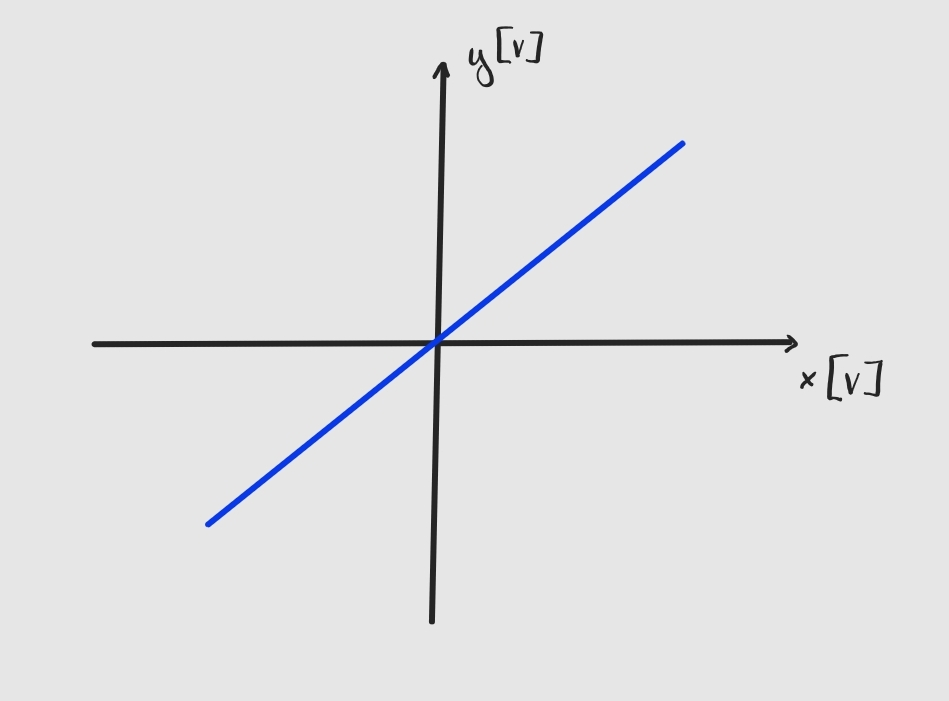
\includegraphics{upornik}
  \caption{\small Skica karakteristike upornika pri $\nu = 50\si{Hz}$}
\end{slika}

\[
  R = \frac{\Delta y}{\Delta x R_{not}} = \frac{3.7\si{V}}{3.75\si{V} \cdot 1k\omega} = (1010 \pm 30) \Omega
\]

\section*{kondenzator}

Preverite frekvenčni razpon, v katerem sta fazi toka in napetosti premaknjeni za $\frac{\pi}{2}$. Določite $C$ iz meritve toka in napetosti pri znani frekvenci. 

\begin{slika}
  \centering
  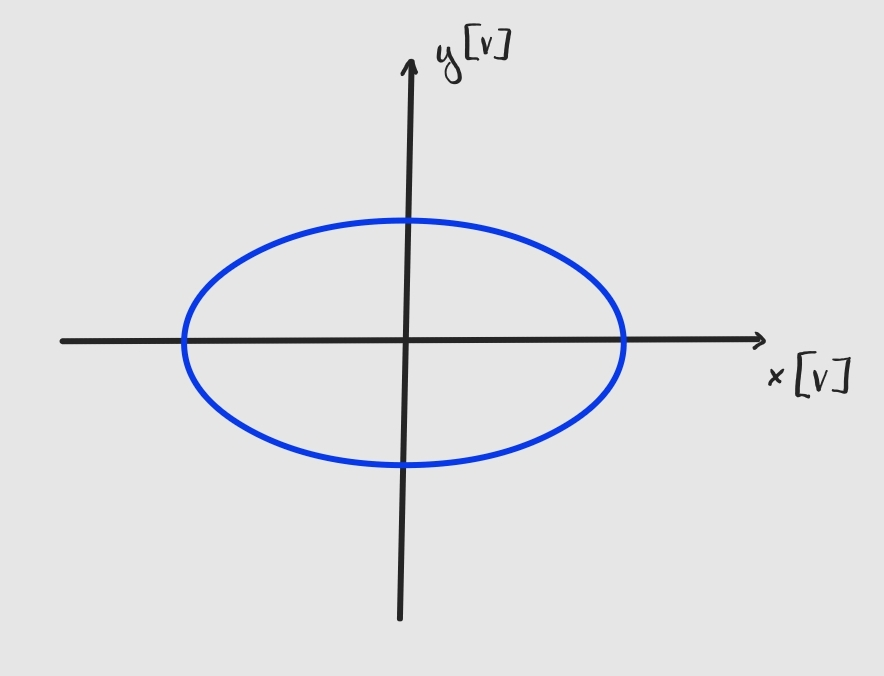
\includegraphics{kondenzator}
  \caption{\small Skica karakteristike kondenzatorja pri $\nu = 50\si{Hz}$}
\end{slika}

Pri faznem zamiku $\frac{\pi}{2}$ velja: 

\[
 C = \frac{\Delta y}{\Delta x R_{not} \omega} = \frac{1.25\si{V}}{3.5\si{V}\cdot 2\pi \cdot 50\si{Hz} \cdot 1k\omega}
\]




\end{document}